%%%%%%%%%%%%%%%%%%%%%%%%%%%%%%%%%%%%%%%%%
% Short Sectioned Assignment
% LaTeX Template
% Version 1.0 (5/5/12)
%
% This template has been downloaded from:
% http://www.LaTeXTemplates.com
%
% Original author:
% Frits Wenneker (http://www.howtotex.com)
%
% License:
% CC BY-NC-SA 3.0 (http://creativecommons.org/licenses/by-nc-sa/3.0/)
%
%%%%%%%%%%%%%%%%%%%%%%%%%%%%%%%%%%%%%%%%%

%----------------------------------------------------------------------------------------
%	PACKAGES AND OTHER DOCUMENT CONFIGURATIONS
%----------------------------------------------------------------------------------------

\documentclass[paper=a4, fontsize=11pt]{scrartcl} % A4 paper and 11pt font size

\usepackage[T1]{fontenc} % Use 8-bit encoding that has 256 glyphs
%\usepackage{fourier} % Use the Adobe Utopia font for the document - comment this line to return to the LaTeX default
\usepackage[english]{babel} % English language/hyphenation
\usepackage{amsmath,amsfonts,amsthm} % Math packages
\usepackage{mathtools} %More math! (For dscases)
\usepackage{hyperref} %HTML package
\usepackage{pgfplots} %Makes plots in LaTeX
\usepackage{tikz} %Also tikz?
\usepackage{bm} %makes vectors bold
\usepackage{bbm} %Blackboard bold 1
\usepgfplotslibrary{fillbetween}%Let's me fill between named plots
\usepackage{graphicx} %import pics
\graphicspath{ {Python_figs/} }
\DeclareGraphicsExtensions{.pdf,.png,.jpg}
\usepackage{sectsty} % Allows customizing section commands
\allsectionsfont{ \normalfont\scshape} % Make all sections the default font and small caps


\renewcommand{\thesubsection}{\alph{subsection}} %Make subsections start with letters

\usepackage{fancyhdr} % Custom headers and footers
\pagestyle{fancyplain} % Makes all pages in the document conform to the custom headers and footers
\fancyhead{} % No page header - if you want one, create it in the same way as the footers below
\fancyfoot[L]{} % Empty left footer
\fancyfoot[C]{} % Empty center footer
\fancyfoot[R]{\thepage} % Page numbering for right footer
\renewcommand{\headrulewidth}{0pt} % Remove header underlines
\renewcommand{\footrulewidth}{0pt} % Remove footer underlines
\setlength{\headheight}{13.6pt} % Customize the height of the header

\numberwithin{equation}{section} % Number equations within sections (i.e. 1.1, 1.2, 2.1, 2.2 instead of 1, 2, 3, 4)
\numberwithin{figure}{section} % Number figures within sections (i.e. 1.1, 1.2, 2.1, 2.2 instead of 1, 2, 3, 4)
\numberwithin{table}{section} % Number tables within sections (i.e. 1.1, 1.2, 2.1, 2.2 instead of 1, 2, 3, 4)

\setlength\parindent{0pt} % Removes all indentation from paragraphs - comment this line for an assignment with lots of text

\usepackage{listings}
\lstset{language=Python}


%----------------------------------------------------------------------------------------
%	TITLE SECTION
%----------------------------------------------------------------------------------------

\newcommand{\horrule}[1]{\rule{\linewidth}{#1}} % Create horizontal rule command with 1 argument of height

\title{	Assignment 1}

\author{Benjamin Jakubowski} % Your name

\date{\normalsize\today} % Today's date or a custom date

\begin{document}

\maketitle % Print the title

%----------------------------------------------------------------------------------------
%	PROBLEM 1
%----------------------------------------------------------------------------------------

\section*{2.2 Gradient Descent Setup}

\subsection*{1. Objective function}

First, let $X \in \mathbb{R}^{m \times d + 1}$ be the "design matrix", where the $i$'th row of $X$ is $x_i$. Let $y = (y_1, \dots, y_m)^T \in \mathbb{R}^{m \times 1}$ be the "response". Then the objective function $J(\theta)$ is
\[J(\theta) = \frac{1}{2m} ||X\cdot \theta - y ||_2 ^2\]

\subsection*{2. Gradient of $J$}

The gradient of $J$ is
\begin{align*}
J(\theta) &= \frac{1}{2m} ||X\cdot \theta - y ||_2 ^2 \\
   &= \frac{1}{2m} (X\cdot \theta - y)^T (X\cdot \theta - y) \\
\implies \qquad{} \nabla_{\theta} J(\theta) &= \frac{1}{2m} 2(X\cdot \theta - y)^T \cdot X \\
    &= \frac{1}{m} (X\cdot \theta - y)^T \cdot X
\end{align*}
   
\subsection*{3. Expression for $J(\theta + \eta \Delta) - J(\theta)$}
We are interested in finding a first-order approximation for  $J(\theta + \eta \Delta) - J(\theta)$. First note (from the taylor expansion) the first-order approximation of $J(\theta_2)$ around $\theta_1$ is
\[J(\theta_2) \approx J(\theta_1) + \nabla_{\theta} J(\theta) ^T (\theta_2 - \theta_1)\]
Thus, with $\theta_2 = \theta + \eta \Delta$ and $\theta_1 = \theta$, we have
\begin{align*}
J(\theta + \eta \Delta) - J(\theta) &= J(\theta) + \nabla_{\theta} J(\theta) ^T (\theta + \eta \Delta - \theta) \\
   &= J(\theta) + \nabla_{\theta} J(\theta) ^T (\eta \Delta) \\
   &= J(\theta) + \eta \nabla_{\theta} J(\theta) ^T \cdot \Delta
\end{align*}
As an intuitive explanation for this result, note $\eta \nabla_{\theta} J(\theta) ^T \cdot \Delta$ is just the directional derivative in the direction of $\Delta$, scaled by the step size.
   
\subsection*{4. Expression for updating $\theta$ in the gradient descent algorithm}

To update $\theta$ in the gradient descent algorithm, we simply use:
\[
\theta \leftarrow \theta - \eta \frac{\nabla_{\theta} J(\theta)}{||\nabla_{\theta} J(\theta)||_2}
\]
where
\[ \nabla_{\theta} J(\theta) =\frac{1}{m} (X\cdot \theta - y)^T \cdot X\]

\subsection*{5. Implementing \texttt{compute\_square\_loss} in python}

See code in appendix.

\subsection*{6. Verifying \texttt{compute\_square\_loss}}

Let
\[ X =
	\begin{bmatrix}
		0 & 1 \\
		2 & 3 
	\end{bmatrix}
\textrm{ and }
y =
	\begin{bmatrix}
		2 \\
		4
	\end{bmatrix}
\]

Then, for 
\[
\theta =
	\begin{bmatrix}
		0 \\
		2
	\end{bmatrix}
\]
\[
J(\theta) = \frac{1}{2\cdot2}
\begin{bmatrix}
	0 & 2
\end{bmatrix}
\begin{bmatrix}
0\\
2
\end{bmatrix}
= \frac{1}{4} \cdot 4 = 1
\]

For 
\[\theta =
	\begin{bmatrix}
		0 \\
		1.5
	\end{bmatrix}
\]
\[
J(\theta) = \frac{1}{2\cdot2}
\begin{bmatrix}
	0.5 & 0.5
\end{bmatrix}
\begin{bmatrix}
0.5\\
0.5
\end{bmatrix}
= \frac{1}{4} \cdot 0.5 = 0.125
\]
These results are confirmed using \texttt{compute\_square\_loss}.

\subsection*{7. Implementing \texttt{compute\_square\_loss\_gradient} in python}

See code in appendix.

\subsection*{8. Verifying \texttt{compute\_square\_loss}}

Again, with X and y as defined in 6, for 
\[
\theta =
	\begin{bmatrix}
		0 \\
		2
	\end{bmatrix}
\]
\begin{align*}
\nabla_{\theta}J(\theta) &= \frac{1}{2} \left(
\begin{bmatrix}
	0 & 1\\
	2 & 3
\end{bmatrix}
\begin{bmatrix}
	0 \\
	2
\end{bmatrix}
-
\begin{bmatrix}
	2 \\
	4
\end{bmatrix}
\right)^T
\begin{bmatrix}
	0 & 1\\
	2 & 3
\end{bmatrix} \\
%%%
   &= 
\frac{1}{2} \left(
\begin{bmatrix}
	2 \\
	6
\end{bmatrix}
-
\begin{bmatrix}
	2 \\
	4
\end{bmatrix}
\right)^T
\begin{bmatrix}
	0 & 1\\
	2 & 3
\end{bmatrix} \\
%%%
   &= 
\frac{1}{2} 
\begin{bmatrix}
	0 & 2
\end{bmatrix}
\begin{bmatrix}
	0 & 1\\
	2 & 3
\end{bmatrix} \\
&=
\frac{1}{2} 
\begin{bmatrix}
	4 & 6
\end{bmatrix} \\
&=
\begin{bmatrix}
	2 & 3
\end{bmatrix}
\end{align*}
These results are confirmed using \texttt{compute\_square\_loss\_gradient}.

%----------------------------------------------------------------------------------------

\section*{2.3 Gradient Checker}

\subsection*{1. Complete \texttt{grad\_checker}}

See code in appendix.

\subsection*{2. Complete generic version of \texttt{grad\_checker}}

See code in appendix.


%----------------------------------------------------------------------------------------

\section*{2.4 Batch Gradient Descent}

\subsection*{1. Complete \texttt{batch\_gradient\_descent}}

See code in appendix.

\subsection*{2. Experimenting with batch gradient descent stepsize}

After implementing \texttt{batch\_gradient\_descent}, the following step sizes were tested: 1, 0.5, 0.1, 0.5, and 0.1. Plots showing the value of the objective function as a function of the number of steps for each step size are shown below: \\
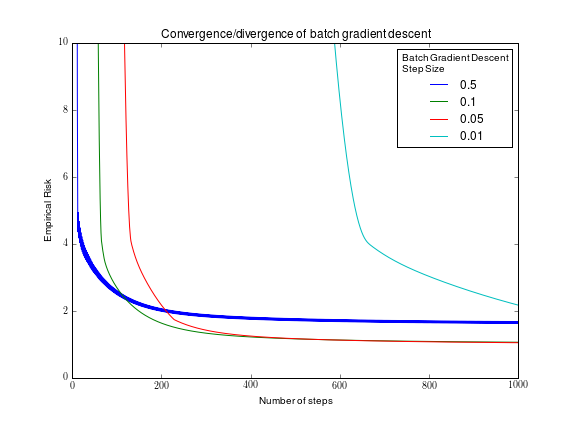
\includegraphics[scale=.8]{./../figures/2_4_2.png} \\
This graph indicates that for this data set:
\begin{itemize}
\item  Batch gradient descent does not converge for $\eta = 0.5$ (note the "thickness" of the blue line indicates oscillation between greater and lower empirical risk values, i.e. across the objective minimum). Additionally $\eta = 0.001$ is too small a step size to achieve convergence in 1000 iterations.
\item Of the tested step sizes, $\eta = 0.1$ converged most quickly, converging to a risk-minimizing $\theta$ within approximately 300 steps.
\end{itemize}
 
 \subsection*{3. Backtracking line search}
 Backtracking line search was implemented in batch gradient descent. Various values for the maximum step size $\alpha_{max}$ were tested, and the search control parameters were both set to 0.5 (per the original Armijo, 1966 paper). The Plots showing the value of the objective function as a function of the number of steps for each $\alpha_{max}$ are shown below:
 
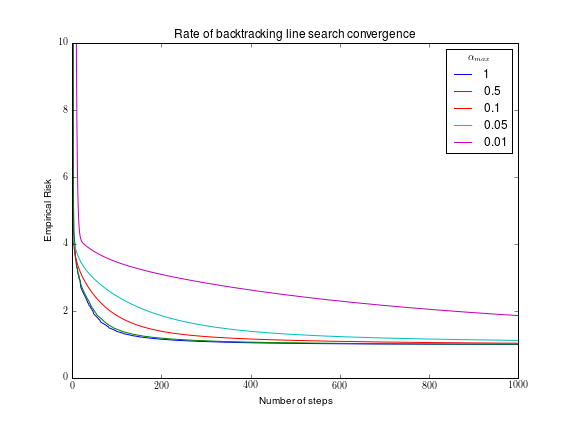
\includegraphics[scale=.65]{./../figures/2_4_3.png} \\
Compared to batch gradient descent with the best fixed step size ($\alpha = 0.1$), it is apparent that backtracking line search converges more quickly:\\
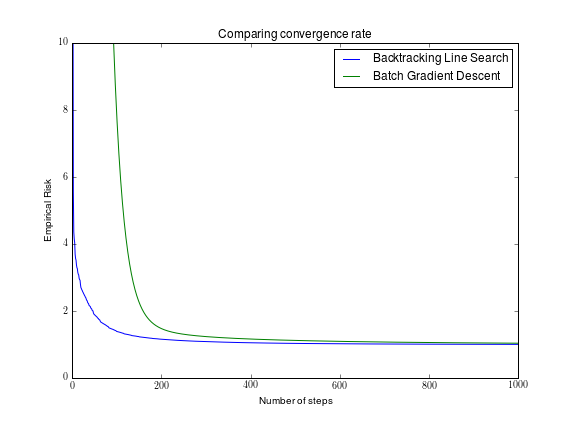
\includegraphics[scale=.65]{./../figures/2_4_3a.png} \\

It is apparent that backtracking line search converges in approximately half the number of steps. However, this improved performance comes at a time cost. Using \texttt{\%timeit} magic in iPython on my machine, the following runtimes were obtained: \\
\begin{center}
\begin{tabular}{|c | c |}
\hline
Method & Runtime \\
\hline
Batch gradient descent ($\alpha = 0.1$) & \texttt{10 loops, best of 3: 20.2 ms per loop} \\
\hline
Backtracking line search & \texttt{10 loops, best of 3: 112 ms per loop} \\
\hline
\end{tabular} \\
\end{center}
 
Thus, given these results, it appears to take approximately 5 times longer to run backtracking line search over batch gradient descent with a fixed step size. Given, however, that the fixed step size was determined empirically by testing multiple different fixed step sizes, backtracking line search produces an improvement in performance in time.

%----------------------------------------------------------------------------------------

\section*{2.5 Ridge Regression}

\subsection*{1. Gradient of $J(\theta)$}

First, note the ridge regression objective function expressed in matrix/vector notation is

\begin{align*}
J(\theta) &= \frac{1}{2m} ||X \theta - y||_2^2 + \lambda ||\theta||_2^2 \\
   &= \frac{1}{2m} (X \theta - y)^T(X \theta - y) + \lambda \theta^T \theta
\end{align*}

Thus, the gradient of $J(\theta)$ is

\[
\nabla_{\theta} J(\theta) = \frac{1}{2m} 2 (X \theta - y)^T X + 2 \lambda \theta = \frac{1}{m} (X \theta - y)^T X + 2 \lambda \theta
\]

Using this gradient, the update rule becomes

\[
\theta \leftarrow \theta - \eta \nabla_{\theta} J(\theta) =  \theta - \eta \left[\frac{1}{m} (X \theta - y)^T X + 2 \lambda \theta \right]
\]

\subsection*{2. Implementing \texttt{compute\_regularized\_square\_loss\_gradient}}

See code in appendix.

\subsection*{3. Implementing \texttt{regularized\_grad\_descent}}

See code in appendix.

\subsection*{4. Decreasing effective regularization of bias term}

To decrease the effective regularization of the bias term, we can increase $B$. To see this, consider the design matrix $X \in \mathbb{R}^{m \times n + 1}$. We can rewrite $X$ as
\[X = \left[D \textrm{  } B \right] \]
where $D$ is the data, and $B$ is the bias vector.

Then, the objective function becomes
\begin{align*}
J(\theta) &= \frac{1}{2m} ||X \theta - y||_2^2 + \lambda ||\theta||_2^2 \\
	&= \frac{1}{2m} || \left[D \textrm{  } B \right] \theta - y||_2^2 + \lambda ||\theta||_2^2
\end{align*}

Now let $B_0$ be given, and let $\theta_0$ be the solution to the ridge regression problem with $X = \left[D \textrm{  } B_0 \right]$.\\

Then, let $B_1 = cB_0$ for some $c >> 1$, and let $\theta_1$ be the ridge regression solution with $X = \left[D \textrm{  } B_1 \right]$. Then it is apparent $\theta_1[n+1] << \theta_0[n+1]$. Thus, by increasing $c$, we can correspondingly decrease the bias coefficient, and in doing see decrease the effective regularization on the bias term such that $\theta[n+1]^2 < \epsilon$ for any $0 < \epsilon$.

\subsection*{5. Finding $\theta_{\lambda}^*$ that minimizes $J(\theta)$}

The following approach was taken to find $\theta_{\lambda}^*$ that minimizes $J(\theta)$:
\begin{enumerate}
\item For candidate $\lambda$'s, batch gradient descent with backtracking line search was used to find the $\theta_{\lambda}$ that minimized the ridge regression loss function.
\item Then, using this $\theta_{\lambda}, \frac{1}{2} MSE$ was calculated for both the training and validation set.
\item Steps 1 and 2 were iterated for increasingly fine-grained $\lambda$ candidate lists, until the optimal $\lambda$ (in the sense of minimum validation loss) was obtained to three decimal places. This yielded $\theta_{\lambda}^*$.
\end{enumerate}
The two plots below show the first two interations:

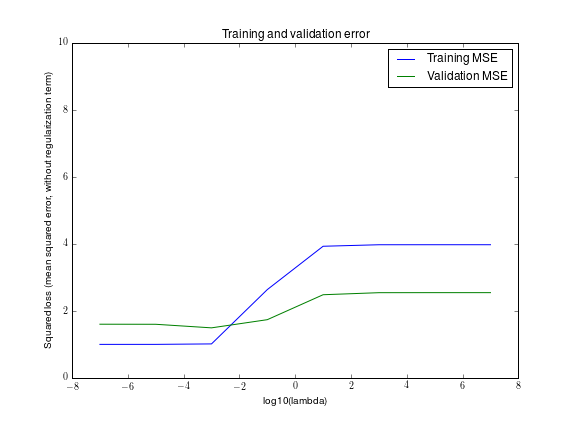
\includegraphics[scale=.6]{./../figures/2_5_5_1.png} \\
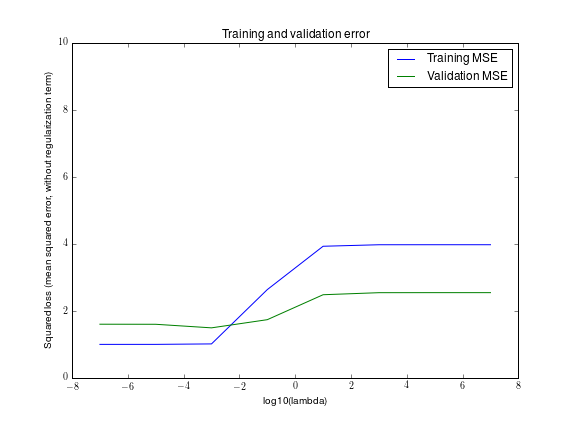
\includegraphics[scale=.6]{./../figures/2_5_5_2.png} \\

Ultimately, the optimal value was $\lambda = .0122$.

\subsection*{6. Comparing different values of B}

Next, setting $\lambda = 0122$, ridge regression with fit with different values of $B$. Plots of $\frac{1}{2}MSE$ on the training and validation set are shown below:

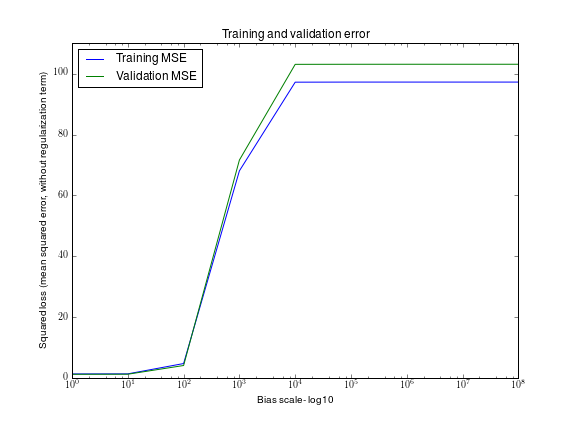
\includegraphics[scale=.8]{./../figures/2_5_6.png} \\

From the plots, it is apparent that regularizing the bias helps the model- the best model has $B=1$, and as $B$ increases (i.e. the regularization on the bias term decreases) the model performance decreases.

\subsection*{7. Average time it takes to compute a single gradient step}

Again, the following runtime for batch gradient descent on $\ell_2$-regularized regression was obtained using \texttt{\%timeit} magic in iPython on my machine:
\begin{center}
\begin{tabular}{|c | c |}
\hline
Method & Runtime \\
\hline
Batch gradient descent for ridge regression& \texttt{10 loops, best of 3: 30.5 ms per loop} \\
\hline
\end{tabular} \\
\end{center}

Since each loop ran with 1000 iterations (steps), each step is computed in approximately $3~\mu$s.

\subsection*{8. Optimal $\theta$ for deployment}

I would choose the $\theta$ fit with $\lambda = 0.012$ and $B = \textbf{1}$. This is because these values minimized the validation set empirical risk. The value of $\theta$ was found, and the first three terms and last term are
\[\begin{bmatrix}-1.13963079  & 0.48238988  & 1.27016416  & \dots & -1.5816435 \end{bmatrix}\]
The remaining coefficients varied between 2.287 and -3.607.

%----------------------------------------------------------------------------------------

\section*{2.5 Stochastic Gradient Descent (SGD)}

\subsection*{1. Update rule for $\theta$ in SGD}

In SGD, the gradient of the risk is approximated by the gradient at a single example. Thus, this gradient (for ridge regression) is

\begin{align*}
\nabla_{\theta} J_{SGD}(\theta) &= \nabla_{\theta} \left[ \frac{1}{2} (x_i^T \cdot \theta - y_i)^2 + \lambda \theta^T \theta \right] \\
	&= (x_i^T \cdot \theta -y) \cdot x_i + 2 \lambda \theta
\end{align*}

Thus, the update rule is
\[
\theta \leftarrow \theta - \eta \left[ (x_i^T \cdot \theta -y) \cdot x_i + 2 \lambda \theta \right]\]

\subsection*{2. Implementing \texttt{stochastic\_grad\_descent}}

See code in appendix.

\subsection*{3. Using SGD to find $\theta_{\lambda}^*$}

In this section, we compare the  convergence of SGD to an optimal $\theta_{\lambda}^*$ using fixed step sizes and step sizes that decrease with the step number. Specifically, fixed step sizes $\eta_t = 0.05$ and 0.005 were tested, along with the following step sizes as functions of t: $\eta_t(t) = \frac{1}{t}$ and $\eta_t(t) = \frac{1}{\sqrt{t}}$. Plots showing the $\ell_2$ regularized square loss for each of these step sizes are shown below:

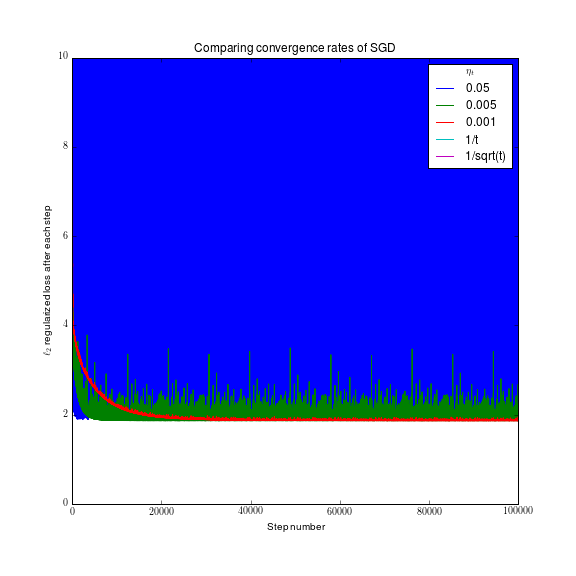
\includegraphics[scale=.8]{./../figures/2_6_3.png}

To compare the results, note:
\begin{itemize}
\item $\eta_t = 0.05$ does not converge- this fixed step size is too large, and as a results we get wild oscillations (resulting in the plot appearing as a solid block).
\item $\eta_t = 0.005$ is somewhat noisy- there is an apparent cycle, with updates of $\theta$ overfitting to the single instance $x_i$, moving $\theta$ away from empirical risk minimizer. 
\item At the resolution selected for the plot above, $\eta_t = 0.001$ appears relatively stable, though at higher resolution we'd expect to observe a similar cycle.
\item Neither $\eta_t = \frac{1}{t}$ or $\eta_t = \frac{1}{\sqrt{t}}$ converge. This is likely due to the initially large step size (i.e. for small $t$ $\eta_t$ is relatively large,  compared to our converging fixed steps size, which is on the order of 0.001). Note this claim is further supported by results in 2.5.4.
\end{itemize}

\subsection*{4. Implementing an additional stepsize function}

Next, we try a step size rule of the form $\eta_t = \frac{\eta_0}{1 + \eta_0 \lambda t}$. Using $\eta_0 \in [10^{-5}, 10^{-4}, ... 10^{1}]$, we obtain the following convergence results:

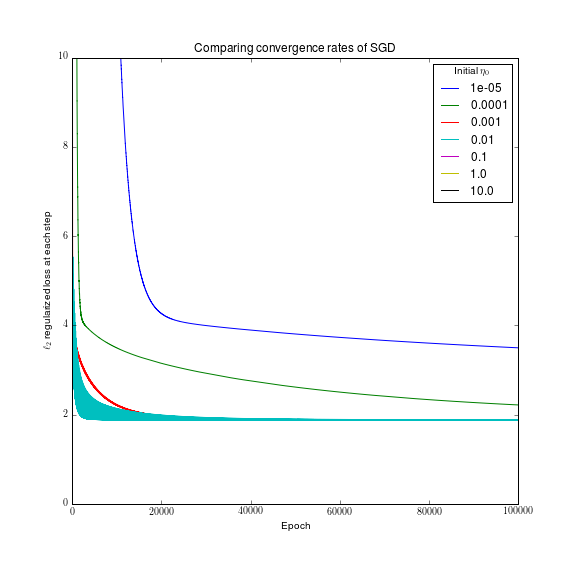
\includegraphics[scale=.8]{./../figures/2_6_4.png}

Comparing these results, it is apparent that the convergence rate increases with $\eta_0$ up to $\eta_0 = 0.01$. However, all tested $\eta_0 \geq 0.1$ diverged.

\subsection*{5. Comparing runtime}

Again, the following runtimes for SGD on $\ell_2$-regularized regression was obtained using \texttt{\%timeit} magic in iPython on my machine:
\begin{center}
\begin{tabular}{|c | c | c |}
\hline
Stepsize & Runtime & Avg. per epoch \\
\hline
0.001 & \texttt{1 loops, best of 3: 2.4 s per loop} & 2.4 ms \\ 
\hline
0.005 & \texttt{1 loops, best of 3: 2.49 s per loop} & 2.49 ms\\
\hline
$1/t$ & \texttt{1 loops, best of 3: 2.92 s per loop} & 2.92 ms \\
\hline
$1/\sqrt{t}$ & \texttt{1 loops, best of 3: 3.07 s per loop} & 3.07 ms \\
\hline
$\frac{\eta_0}{1 + \eta_0 \lambda t}, \textrm{ with } \eta_0 = 0.1$ & \texttt{1 loops, best of 3: 2.68 s per loop} & 2.68 ms \\
\hline
\end{tabular} \\
\end{center}

\subsection*{6. Comparing SGD and Gradient Descent}

First, lets compare the convergence rate. Plots of $log_{10}$(Empirical Risk) ($\ell_2$ regularized risk on the entire training set) are shown for several versions of SGD and Gradient Descent (all with $\lambda_{reg} = 0.0122$, as discussed previously).

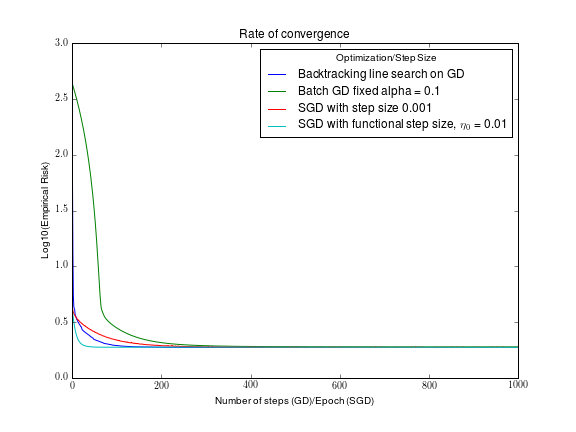
\includegraphics[scale=.7]{./../figures/2_6_6.png}

From this plot, it appears optimal convergence is obtained using SGD with functional step size $\eta_t = \frac{\eta_0}{1 + \eta_0 \lambda t} = \frac{0.01}{1 + 0.01 \lambda t}$. However, batch GD with backtracking line search achieves similar convergence.
\\

Next, let's compare runtimes. Using \texttt{\%timeit}, we observed a step in SGD was on the order of $3~\mu$s (with backtracking line search increasing runtime by approximately $5\times$), while an epoch in SGD was on the order of 3 ms. This indicates an epoch of SGD is on the order of 1000 times slower than a step of SGD. This, however, is not unexpected- our implementation of SGD evaluates the loss (over the entire training set) at each step. This is anticipated to substantially increase runtime. 

Regardless, as implemented, I would select the following constraints:

\begin{center}
\begin{tabular}{|c | c |}
\hline
Constraint & Algorithm \\
\hline
Minimized total time & Batch gradient descent with backtracking line search \\
\hline
Minimized total number of steps/epochs & SGD with functional step size, $\eta_0 = 0.01$ \\
\hline
\end{tabular}
\end{center}

%----------------------------------------------------------------------------------------

\section*{3. Risk Minimization}

\subsection*{1. Posterior Mean: Minimum MSE estimator}

Let $f$ be an arbitrary decision function, and let $x$ be given. Then, conditioning on $X = x$,

\begin{align*}
\frac{1}{2} E \left[ \left( Y - f(X) \right) ^2 | X = x \right ] =& \frac{1}{2} E \left[ \left( Y - E[Y|X] + E[Y|X] - f(X) \right) ^2 | X = x \right] \\
	=& \frac{1}{2} E \left[ \left( Y - E[Y|X] \right) ^2 | X = x \right] + \frac{1}{2} E \left[ \left( E[Y|X] - f(X) \right) ^2 | X = x \right]\\
	& + E \left[ ( Y - E[Y|X]) (E[Y|X] - f(X))  | X = x \right] \\
\end{align*}
Next, noting the last term $E \left[ ( Y - E[Y|X]) (E[Y|X] - f(X))  | X = x \right] = 0$ yields:
\[\frac{1}{2}  E \left[ \left( Y - f(X) \right) ^2 | X = x \right] = \frac{1}{2}  E \left[ \left( Y - E[Y|X] \right) ^2 | X = x \right] +\frac{1}{2}  E \left[ \left( E[Y|X] - f(X) \right) ^2 | X = x \right] \]

Next, by the non-negativity of expectation, we have
\begin{align*}
\frac{1}{2}  E \left[ \left( Y - f(X) \right) ^2 | X = x \right] &= \frac{1}{2}  E \left[ \left( Y - E[Y|X] \right) ^2 | X = x \right] +\frac{1}{2}  E \left[ \left( E[Y|X] - f(X) \right) ^2 | X = x \right] \\
	& \geq \frac{1}{2}  E \left[ \left( Y - E[Y|X] \right) ^2 | X = x \right] \\
\end{align*}

Finally, using iterated expectations, we have

\begin{align*}
E\left[ \frac{1}{2}  E \left[ \left( Y - f(X) \right) ^2 | X \right]\right] &\geq \left[\frac{1}{2}  E \left[ \left( Y - E[Y|X] \right) ^2 | X = x \right]\right] \\
\implies \qquad{} \frac{1}{2}  E \left[ \left( Y - f(X) \right) ^2 \right] & \geq \frac{1}{2}  E \left[ \left( Y - E[Y|X] \right) ^2 \right]
\end{align*}

Hence the conditional expectation minimizes the mean squared error.


%----------------------------------------------------------------------------------------

\end{document}